\documentclass[a4paper,12pt]{article}

\usepackage[
    left=2cm,
    right=2cm,
    top=3cm,
    bottom=3cm
]{geometry}

\usepackage[utf8]{inputenc}
\usepackage[czech]{babel}
\usepackage[T1]{fontenc}
\usepackage{graphicx}
\usepackage{array}
\usepackage{booktabs}
\usepackage{tabularx}
\usepackage{makecell}
\usepackage{float}
\usepackage{newunicodechar}
\usepackage{url}
\usepackage{siunitx}
\usepackage{listings}
\usepackage{xcolor}
\usepackage{diagbox}
\usepackage{hyperref}
\usepackage{tikz}
\usepackage{pgfplots}
\pgfplotsset{compat=1.18}

\usepackage{fancyhdr}
\pagestyle{fancy}

\fancyhf{}
\fancyhead[L]{Měření teplotního součinitele délkové roztažnosti}
\fancyhead[R]{Pavel Pernička}
\fancyfoot[C]{\thepage}

\fancypagestyle{firstpage}{
    \fancyhf{}
    \renewcommand{\headrulewidth}{0pt}
    \renewcommand{\footrulewidth}{0pt}
    \fancyfoot[C]{\thepage}
}

\definecolor{myblue}{RGB}{111,0,248}
\newcommand{\colorcircle}[1]{%
  \tikz[baseline=-0.6ex]\draw[fill=#1,draw=none] (0,0) circle (1.5ex);%
}
\newcommand{\unitC}{\,^\circ\mathrm{C}}
\newcommand{\unitV}{\,\mathrm{V}}
\newcommand{\unitA}{\,\mathrm{A}}
\newcommand{\units}{\,\mathrm{s}}
\newcommand{\unitmin}{\,\mathrm{min}}

\newcommand{\centered}[1]{\begin{tabular}{l} #1 \end{tabular}}

\addto\captionsczech{\renewcommand{\refname}{Seznam použité literatury}}
\addto\captionsczech{\renewcommand{\figurename}{\textbf{Obrázek}}}
\addto\captionsczech{\renewcommand{\tablename}{\textbf{Tabulka}}}
\renewcommand{\lstlistingname}{\textbf{Kód}}

\lstset{
    language=Python,
    basicstyle=\ttfamily\footnotesize,
    keywordstyle=\color{blue},
    commentstyle=\color{gray},
    stringstyle=\color{red},
    numbers=left,
    numberstyle=\tiny\color{gray},
    stepnumber=1,
    breaklines=true,
    frame=single
}

\begin{document}
\thispagestyle{firstpage}

\vspace*{\fill}
\begin{center}
\renewcommand{\arraystretch}{1.75}

\begin{tabularx}{\textwidth}{|X|X|X|}
    \hline
    \multicolumn{1}{|c|}{\rule{0pt}{2.25cm} 
\includegraphics[height=2cm]{img/ctu_logo.png}}
    & \multicolumn{2}{c|}{\makecell{\textbf{KATEDRA FYZIKY}}} \\
    \hline
    \multicolumn{3}{|c|}{\Large \textbf{\centered{LABORATORNÍ CVIČENÍ Z FYZIKY}}} \\
    \hline
    \multicolumn{2}{|X}{\small{Jméno} \newline \textbf{Pavel Pernička}}
    & \multicolumn{1}{|X|}{\small{Datum měření} \newline \textbf{16.12.2025}} \\
    \hline
    {\small{Semestr} \newline \textbf{Zimní 2025}}
    & {\small{Ročník} \newline \textbf{2.}}
    & {\small{Datum odevzdání} \newline \textbf{23.12.2025}} \\
    \hline
    {\small{Stud. skupina} \newline \textbf{6}}
    & {\small{Lab. skupina} \newline \textbf{1061}}
    & {\small{Klasifikace} \newline} \\
    \hline
    \multicolumn{3}{|c|}{\rule{0pt}{1cm}} \\
    \hline
    \multicolumn{1}{|X|}{\small{Číslo úlohy \newline \textbf{9}}}
    & \multicolumn{2}{|p{9cm}|}{\small{Název úlohy \newline \textbf{Měření teplotního součinitele délkové roztažnosti -- hodnoty}}} \\
    \hline
\end{tabularx}

\end{center}
\vspace*{\fill}

\newpage
\section{Úkol měření}
\begin{itemize}
    \item Stanovte teplotní součinitel délkové roztažnosti pro alespoň dva různé materiály.
    \item Pro měřené vzorky zhotovte graf závislosti jejich prodloužení na změně teploty.
\end{itemize}


\section{Seznam použitých přístrojů}
\begin{itemize}
    \item Čerpadlo s ohřívačem a nádobou na vodu
    \item Teploměr pro teplotu vody v nádobě
    \item Lavice pro uchycení testovaného vzorku
    \item Testované vzorky kovů s kanálkem pro cirkulaci vody
    \item Měřič prodloužení vzorku
    \item Kýbl na vypouštění vody
\end{itemize}

\section{Postup měření}
\begin{itemize}
    \item Do nádoby nalijeme vodu z kohoutku cca 2 cm pod okraj.
    \item Vzorek zasadíme do testovací lavice a připneme hadičky
    \item Namontujeme měřič prodloužení vzorku
    \item Zapneme čerpadlo a na termostatu nastavíme teplotu tak, aby nedocházelo k ohřevu
    \item Necháme chvíli cirkulovat vodu, abychom měli vzorek na iniciální teplotě. Následně odečteme teplotu a počáteční hodnotu na měřiči prodloužení.
    \item Postupně po krocích o velikosti $5\ \unitC$ zvyšujeme teplotu na termostatu a zaznamenáváme prodloužení.
\end{itemize}

\newpage
\section{Naměřené hodnoty}

\subsection{Hliníkový vzorek}

\begin{table}[H]
\centering
\renewcommand{\arraystretch}{1.5}
\begin{tabular}{|c|c|c|}
\hline
$n$ & $l_n$ [mm] & $t_n$ [°C] \\
\hline
0 & 0{,}05 & 23{,}9 \\
1 & 0{,}15 & 29{,}4 \\
2 & 0{,}23 & 34{,}7 \\
3 & 0{,}30 & 39{,}7 \\
4 & 0{,}34 & 44{,}6 \\
5 & 0{,}45 & 49{,}6 \\
6 & 0{,}50 & 54{,}6 \\
7 & 0{,}56 & 59{,}6 \\
\hline
\end{tabular}
\caption{Naměřené hodnoty závislosti prodloužení $l_n$ na teplotě $t_n$ pro hliník}
\label{tab:hlinik}
\end{table}


\subsection{Mosazný vzorek}

\begin{table}[H]
\centering
\renewcommand{\arraystretch}{1.5}
\begin{tabular}{|c|c|c|}
\hline
$n$ & $l_n$ [mm] & $t_n$ [°C] \\
\hline
0 & 0{,}04 & 27{,}7 \\
1 & 0{,}10 & 32{,}7 \\
2 & 0{,}16 & 39{,}7 \\
3 & 0{,}24 & 42{,}7 \\
4 & 0{,}29 & 47{,}7 \\
5 & 0{,}35 & 52{,}7 \\
6 & 0{,}40 & 57{,}7 \\
7 & 0{,}45 & 62{,}7 \\
\hline
\end{tabular}
\caption{Naměřené hodnoty závislosti prodloužení $l_n$ na teplotě $t_n$ pro mosaz}
\label{tab:mosaz}
\end{table}


\newpage
\section{Zpracování naměřených hodnot}
Abychom mohli určit koeficient délkové roztažnosti, nejprve převedeme naměřené teploty $t_n$ a~prodloužení $l_n$ na jejich změny $\Delta l$ a $\Delta t$.

$$
\Delta l_n = l_n - l_{n-1}, \qquad
\Delta t_n = t_n - t_{n-1}
$$

\begin{table}[H]
\centering
\renewcommand{\arraystretch}{1.5}
\begin{tabular}{|c|c|c|c|c|}
\hline
 & \multicolumn{2}{c|}{\textbf{Hliník}} & \multicolumn{2}{c|}{\textbf{Mosaz}} \\
\hline
$n$ & $\Delta l_n$ [mm] & $\Delta t_n$ [°C]
    & $\Delta l_n$ [mm] & $\Delta t_n$ [°C] \\
\hline
1 & 0{,}10 & 5{,}5 & 0{,}06 & 5{,}0 \\
2 & 0{,}08 & 5{,}3 & 0{,}06 & 7{,}0 \\
3 & 0{,}07 & 5{,}0 & 0{,}08 & 3{,}0 \\
4 & 0{,}04 & 4{,}9 & 0{,}05 & 5{,}0 \\
5 & 0{,}11 & 5{,}0 & 0{,}06 & 5{,}0 \\
6 & 0{,}05 & 5{,}0 & 0{,}05 & 5{,}0 \\
7 & 0{,}06 & 5{,}0 & 0{,}05 & 5{,}0 \\
\hline
\end{tabular}
\caption{Změny prodloužení $\Delta l_n$ a teploty $\Delta t_n$ vypočítané z původních dat}
\label{tab:delta_krokova}
\end{table}



\section{Určení koeficientu délkové roztažnosti}
Při výpočtu budeme pracovat s průměrnými hodnotami změny délky $\bar{\Delta l}$ a teploty $\bar{\Delta t}$:

$$
\bar{\Delta l} = \frac{1}{N} \sum_{i=0}^N \Delta l \qquad \bar{\Delta t} = \frac{1}{N} \sum_{i=0}^N \Delta t
$$

Tyto hodnoty pak dosadíme do vztahu pro výpočet samotného koeficientu:

$$
\alpha = \frac{1}{l_0}\cdot \frac{\bar{\Delta l}}{\bar{\Delta t}}
$$

Dosazením získáváme hodnoty:
$$
\alpha_{Al} = 2{,}38 \cdot 10^{-5}\,\mathrm{K}^{-1} \quad \text{(Hliník)}
$$

$$
\alpha_{CuZn} = 1{,}95 \cdot 10^{-5}\,\mathrm{K}^{-1} \quad \text{(Mosaz)}
$$


\section{Grafy}

\begin{figure}[H]
\centering
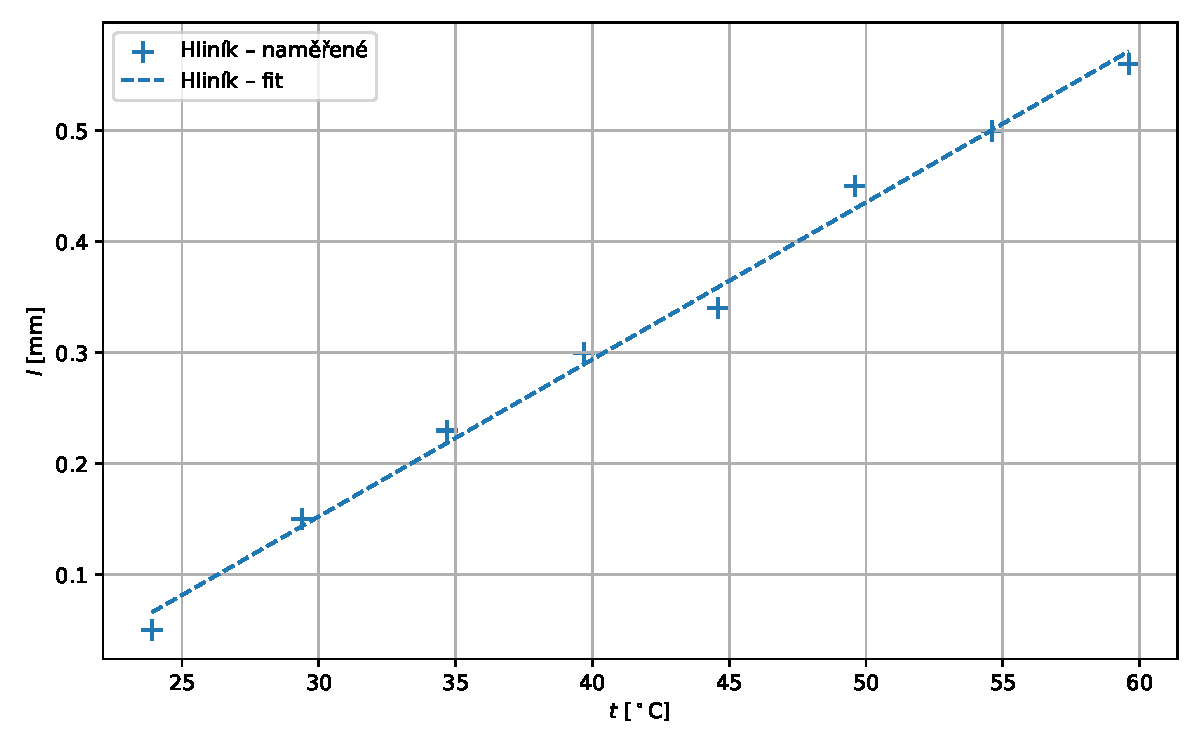
\includegraphics[width=0.92\textwidth]{img/al.pdf}
\caption{Závislost prodloužení hliníkového vzorku na teplotě}
\end{figure}

\begin{figure}[H]
\centering
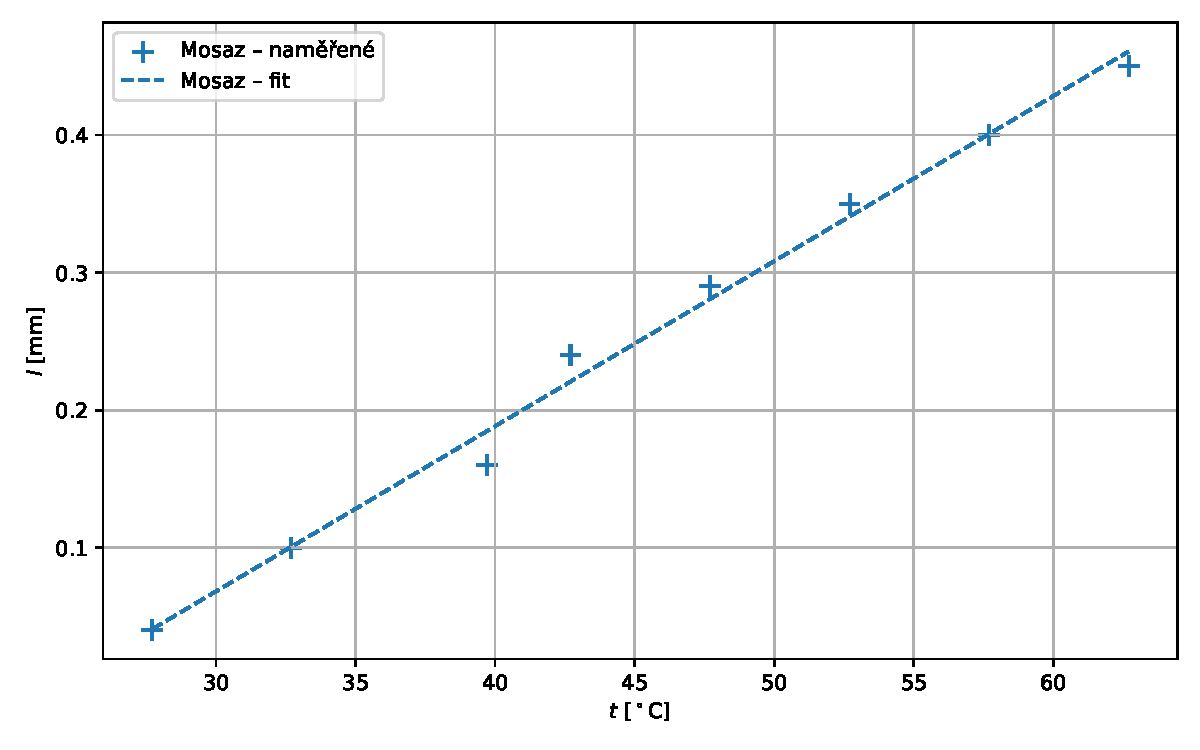
\includegraphics[width=0.92\textwidth]{img/cuzn.pdf}
\caption{Závislost prodloužení mosazného vzorku na teplotě}
\end{figure}

\section{Závěr}
Pro hliníkový vzorek jsme vypočítali koeficient délkové roztažnosti $\alpha_{Al} = \mathbf{23,8} \cdot 10^{-6}\,\mathrm{K}^{-1}$ a pro mosazný vzorek $\alpha_{CuZn} = \mathbf{19,5} \cdot 10^{-6}\,\mathrm{K}^{-1}$. Pokud tyto hodnoty srovnáme s tabulkou ze zadání, zjistíme, že jsme se s rozumnou odchylkou trefili. 

\begin{table}[H]
\centering
\renewcommand{\arraystretch}{1.5}
\begin{tabular}{|l|c||l|c|}
\hline
\textbf{Materiál} & $\boldsymbol{\alpha\ [10^{-6}\ ^\circ C^{-1}]}$
& \textbf{Materiál} & $\boldsymbol{\alpha\ [10^{-6}\ ^\circ C^{-1}]}$ \\
\hline
tavený křemen   & 0{,}5 & beton    & 12 \\
Invar           & 1{,}6 & měď      & 17 \\
sklo (obyčejné) & 8{,}5 & \textbf{mosaz}    & \textbf{19} \\
ocel            & 11    & \textbf{hliník}   & \textbf{23} \\
\hline
\end{tabular}
\caption{Tabulkové hodnoty teplotního součinitele délkové roztažnosti vybraných materiálů ze zadání}
\label{tab:alpha_tabulkove}
\end{table}


\newpage
\section{Přílohy}
\begin{itemize}
    \item Foto záznamového papíru s hodnotami
\end{itemize}

\begin{thebibliography}{}

    \bibitem{zadani}
    Milan Červenka. \textit{Měření teplotního součinitele délkové roztažnosti}. Laboratorní úloha, 2015. Dostupné online: \url{https://planck.fel.cvut.cz/praktikum/downloads/navody/roztaznost.pdf}.

    \bibitem{skripta}
    Michal Bednařík. \textit{Studijní texty k předmětu Fyzika 2}.
    
    \bibitem{zpracdat}
    Milan Červenka. \textit{Zpracování fyzikálních měření}. Studijní text pro fyzikální praktikum, 2020. Dostupné online: \url{https://planck.fel.cvut.cz/praktikum/downloads/navody/zpracdat.pdf}.

\end{thebibliography}

\end{document}
